% 06-trainingsablauf.tex
\section{Trainingsablauf in Isaac}
\label{sec:trainingsablauf}

Wie in Phase~1 gezeigt, ist es von Vorteil, das \ac{RL}-Training nicht ohne Vorbereitung zu starten. Ein Kamera-Agent, der von Null an lernt, muss zwei Dinge gleichzeitig herausfinden: was die Pixel bedeuten und wie man fährt. Das einzige Signal dafür ist die Belohnung. Um das zu erleichtern, wird der Bildteil des Netzes vorab überwacht trainiert. Anschließend folgen die beiden fahrenden Kamera-Agenten, die im Verlauf der Arbeit entstanden sind, im Folgenden Agent~1 und Agent~2. Beide durchlaufen dieselben vier Stufen, unterscheiden sich aber im Ziel des Vortrainings und in den Darstellungen der Strecke: Agent~1 lernt auf einer einzigen Darstellung, Agent~2 auf zwölf.

\subsection{Die Trainingspipeline in 3D}
\label{sec:pipeline3d}

Entsprechend der Python-Umgebung wird auch hier eine mehrstufige Trainingspipeline verwendet, um den Ablauf des \ac{RL}-Trainings effizienter zu gestalten. Diese Pipeline besteht aus vier separaten Stufen, wie in Abbildung~\ref{fig:pipeline_stufen} zu sehen.

\begin{figure}[htbp]
  \centering
  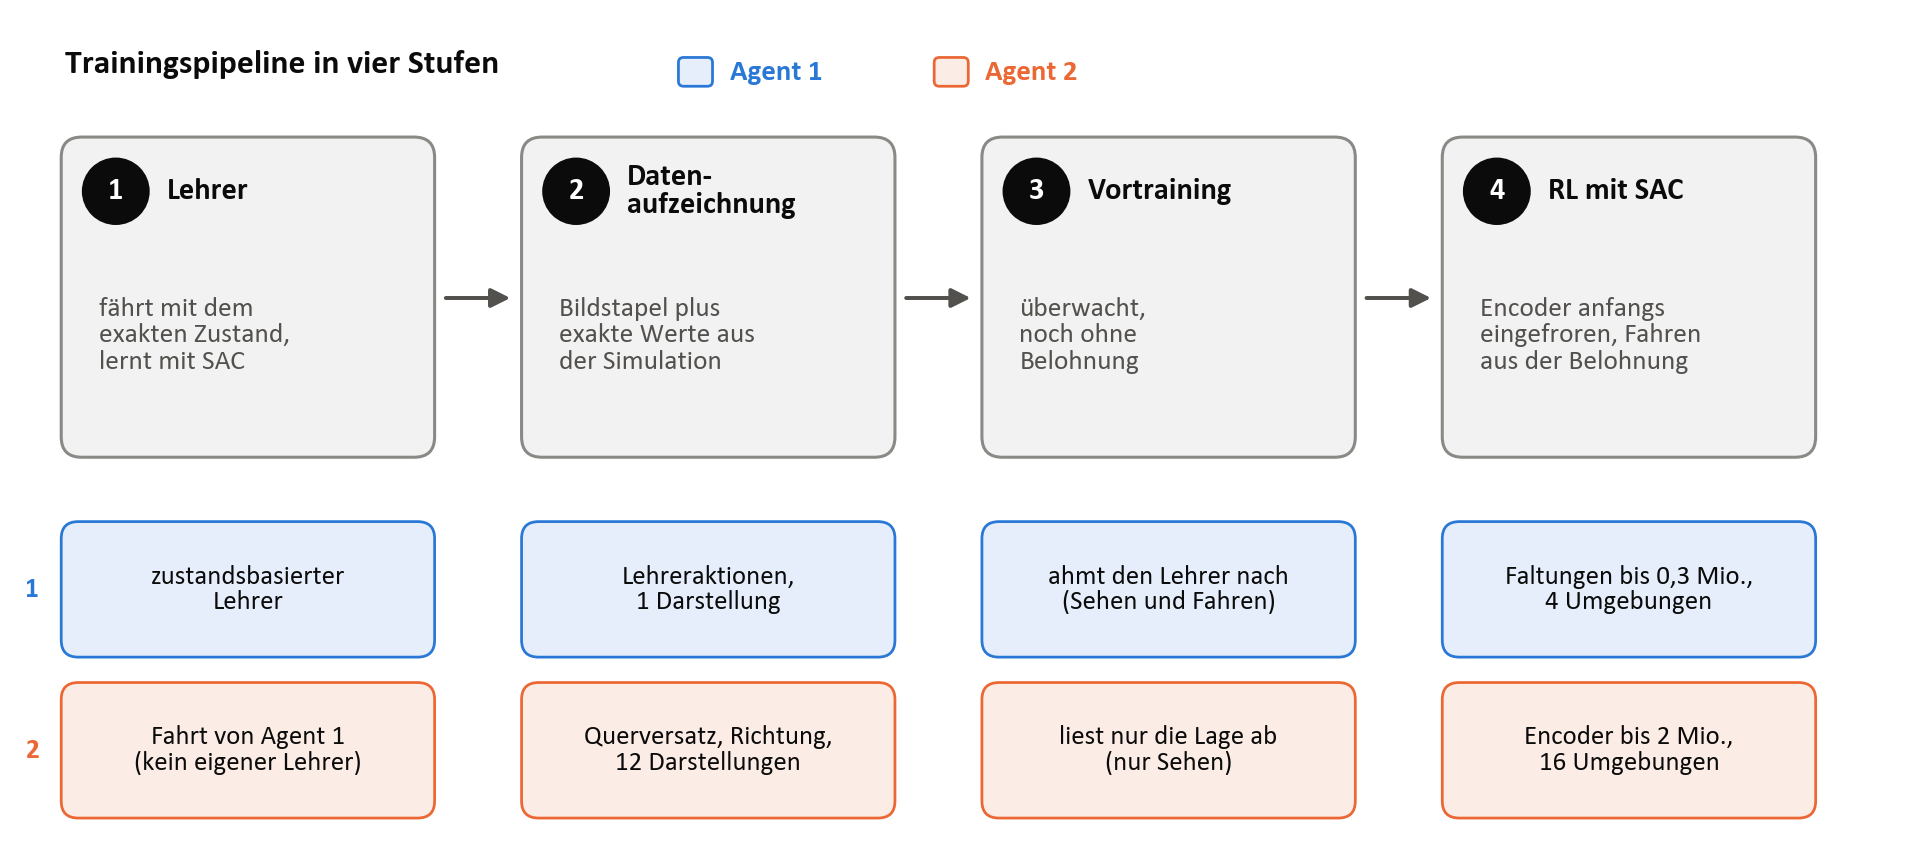
\includegraphics[width=\linewidth]{chapters/felix_teil/bilder/pipeline_stufen.png}
  \caption{Trainingspipeline in vier Stufen. Oben der gemeinsame Ablauf, darunter die Unterschiede zwischen Agent~1 (blau) und Agent~2 (orange).}
  \label{fig:pipeline_stufen}
\end{figure}

\paragraph{Stufe 1 -- Lehrer.}
Wie in Phase~1 wird zuerst ein Agent trainiert, der als Lehrer für den späteren bildbasierten Agenten dient (Abschnitt~\ref{subsec:privileged}). Während der Lehrer in der 2D-Umgebung anhand von Lidar-Strahlen lernte, ist er hier zustandsbasiert. Er erhält den exakten Zustand aus der Simulation, also Geschwindigkeit, Drehrate, Richtungsfehler, Querversatz und die Abstände zu beiden Fahrbahnkanten, sowie seine letzte Aktion. Da Isaac alle diese Größen ohnehin kennt, ist es nicht nötig, Abstandsstrahlen nachzubilden.

Dieser Lehrer wird mit \ac{SAC} auf 64 parallelen Umgebungen trainiert und fährt nach \num{768000} Übergängen 8 Runden je Episode ohne Crash, mit einer Rundenzeit von ca.\ \SI{8.3}{\second}. Damit ist gezeigt, dass Physik und Belohnungsfunktion in 3D lösbar sind.

\paragraph{Stufe 2 -- Datenaufzeichnung.}
Anschließend fährt der Lehrer in der Kamera-Umgebung. Zu jedem Schritt werden der Bildstapel und die Aktion des Lehrers gespeichert, insgesamt \num{48000} Paare. Abweichend von Phase~1 fährt der Lehrer dabei deterministisch, ohne injiziertes Rauschen (Gleichung~\eqref{eq:noise}), Vielfalt im Datensatz entsteht nur durch die zufälligen Startpositionen. Für Agent~2 stammen die Bilder stattdessen aus einer Fahrt von Agent~1, die in allen zwölf Darstellungen der Strecke gerendert wird (Abschnitt~\ref{sec:agent2}).

\paragraph{Stufe 3 -- Vortraining.}
Vortrainiert wird der Teil des Netzes, der aus dem Bildstapel Merkmale berechnet, im Folgenden Merkmalsextraktor (Encoder). Er besteht wie in Phase~1 aus den drei Faltungsschichten des NatureCNN \cite{mnih2015human} und einer voll verbundenen Schicht mit 512 Neuronen. Für Agent~1 lernt das Netz analog zu Phase~1, die Aktionen des Lehrers nachzuahmen (\ac{BC}, Abschnitt~\ref{subsec:il}). Bestätigt wurde dabei die Warnung aus Abschnitt~\ref{sec:ergebnisse_pipeline}, dass ein niedriger Vorhersagefehler kein Fahrkönnen belegt: Von zwei Netzen fuhr das mit dem schlechteren Fehler ($R^2 = \num{0.25}$ gegen \num{0.47}) \SI{60}{\percent} weiter. Nach dem Vorhersagefehler wäre das schlechtere Netz ausgewählt worden. Vortrainierte Netze wurden deshalb im Fahrversuch bewertet, nicht am Verlust.

Für Agent~2 lernt der Encoder dagegen nicht die Aktionen, sondern nur die Lage des Fahrzeugs, Querversatz zur Mittellinie und Richtungsfehler, beide aus der Simulation exakt bekannt. Vortrainiert wird damit nur das Sehen, nicht das Fahren, wie auf eine Situation zu reagieren ist, lernt der Agent erst im \ac{RL}-Training.

\paragraph{Stufe 4 -- Online-Training mit SAC.}
Die vortrainierten Gewichte werden in das Netz des \ac{RL}-Agenten übertragen und als Grundlage für das \ac{SAC}-Training verwendet. Für Agent~1 werden nur die Faltungsschichten übernommen, für Agent~2 der gesamte Encoder. Der Kopf hinter dem Encoder, der aus den Merkmalen die Aktionen und ihre Bewertung berechnet, ist zu Beginn zufällig initialisiert.

Gerade am Anfang des Trainings sind die Gradienten des Reinforcement Learning stark verrauscht, der Agent verlässt nach wenigen Schritten die Fahrbahn, und der Critic kann den Wert einer Aktion kaum einschätzen. Lernt der Encoder in dieser Phase mit, überschreiben diese Gradienten das vortrainierte Sehen, bevor der Kopf gelernt hat, es zu nutzen.

Der Encoder wird deshalb zu Beginn eingefroren: Seine Gewichte bleiben für eine festgelegte Zahl von Übergängen unverändert, und nur der Kopf lernt. Danach wird der Encoder aufgetaut und lernt mit. Die Gradienten verfeinern das Sehen nun, statt es zu zerstören. Bei Agent~1 waren die Faltungsschichten bis \num{0.3}~Mio.\ Übergänge eingefroren, bei Agent~2 der gesamte Encoder bis 2~Mio. Wie entscheidend dieser Schritt ist, zeigt ein Gegenversuch (Abschnitt~\ref{sec:einfrieren}).

\subsection{Training des Kamera-Agenten}
\label{sec:kamera_training}

Der Kamera-Agent wird, wie in Phase~1 erarbeitet, mit \ac{SAC} trainiert (Abschnitte~\ref{subsec:ppo_sac} und~\ref{subsec:ppo_sac_vergleich}); auch die Netzarchitektur, das NatureCNN, stammt aus Phase~1. Actor und Critic besitzen jeweils einen eigenen Encoder, dahinter je einen Kopf, der die drei Aktionen bzw.\ deren Bewertung berechnet.

Während des Trainings fährt der Agent parallel in mehreren Umgebungen. Jeder Übergang landet im Erfahrungsspeicher, aus dem nach jedem Simulationsschritt Stichproben für die Updates gezogen werden. Die Aktionen sind dabei zufällig gestreut, damit der Agent erkundet.

Als Eingabe erhält der Agent ausschließlich den Bildstapel. Belohnung, frühere Aktionen oder die Geschwindigkeit werden nicht zurückgeführt, die Belohnung dient nur als Lernsignal für den Critic.

\paragraph{Bewertung.}
Die Agenten werden nach dem Training deterministisch bewertet, also ohne Zufallsanteil der Aktionen und ohne Bildstörungen, mit zufälligen Startpositionen und getrennt je Darstellung der Strecke. Dabei werden Runden je Episode, mittleres Tempo, beste Rundenzeit und der Anteil der Episoden, die mit einem Crash enden, gemessen. Die Werte aus dem Training eignen sich dafür nicht, weil die Aktionen dort zufällig gestreut und über alle Darstellungen gemittelt sind. Da gute Agenten in \SI{66.67}{\second} das Zeitlimit von etwa sechs Runden erreichen, wurden die fertigen Modelle zusätzlich mit \SI{200}{\second} langen Episoden gemessen.

\subsection{Probleme auf dem Weg zum ersten Agenten}
\label{sec:probleme_agent1}

Bis zum ersten fahrenden Kamera-Agenten vergingen etwa \SI{125}{\hour} Rechenzeit in Läufen, die nichts lernen konnten. Die wesentlichen Fehler traten ohne Absturz oder Warnung auf. Mehrere Fehler betrafen die Vortrainingskette: invertierte Lehrerbilder, Lehreraktionen außerhalb des gültigen Wertebereichs und das Speichern der letzten statt der besten Trainingsepoche.

Auch mit korrektem Bild lernte der Agent zunächst nicht zu fahren. Zum einen bestand eine Belohnungsfalle: Ohne den Fortschrittsterm brachte Geradeausfahren erst ab \SI{0.52}{\meter\per\second} Pluspunkte, sodass ein schnelles Verlassen der Fahrbahn für den Agenten günstiger war als langsames Weiterfahren. Erst der Fortschrittsterm (Abschnitt~\ref{subsec:3d_belohnung}) beseitigte diese Falle. Zum anderen verlor der Agent seine vortrainierte Sehfähigkeit. Das vortrainierte Netz fuhr allein 120 Schritte weit, der Agent nach \num{762000} Übergängen nur noch 44 und damit kürzer als ein Fahrzeug, das ohne Lenken 86 Schritte weit fährt. Das \ac{RL} hatte die vortrainierten Merkmale überschrieben.

\subsection{Einfrieren des Encoders}
\label{sec:einfrieren}

Wie wichtig das Einfrieren des Encoders ist, zeigt ein Gegenversuch: zwei Läufe mit identischem Aufbau, einmal mit eingefrorenem Encoder bis 2~Mio.\ Übergänge und einmal ohne Einfrieren. Der Aufbau entspricht dem von Agent~2 (Abschnitt~\ref{sec:agent2}).

Neben der Episodenlänge werden dafür zwei Kennzahlen aufgezeichnet, beide auf einer Stichprobe von Bildern aus dem Erfahrungsspeicher. Die erste ist der Anteil inaktiver Neuronen der 512er-Schicht, also der Neuronen, die für alle Bilder der Stichprobe null ausgeben. Ein solches Neuron trägt keine Information über das Bild mehr, ist fast die gesamte Schicht inaktiv, erreicht den Kopf des Netzes kaum noch Bildinformation. Die zweite ist die Streuung des Lenkbefehls über die Bilder der Stichprobe. Ist sie null, gibt der Agent für jedes Bild denselben Lenkbefehl aus, er ist blind. In den üblichen Trainingskurven ist beides nicht zu erkennen, sie verlaufen lediglich flach. Tabelle~\ref{tab:gegenversuch_einfrieren} und Abbildung~\ref{fig:gegenversuch_einfrieren} zeigen den Verlauf.

\begin{table}[htbp]
  \centering
  \caption{Gegenversuch Einfrieren, Werte im Trainingsverlauf (Episodenlänge in Schritten / Anteil inaktiver Neuronen der 512er-Schicht / Streuung des Lenkbefehls).}
  \label{tab:gegenversuch_einfrieren}
  \small
  \begin{tabular}{@{}l c c@{}}
    \toprule
    \textbf{Übergänge} & \textbf{ohne Einfrieren} & \textbf{eingefroren bis 2~Mio.} \\
    \midrule
    \num{0.5}~Mio.  & 33 / \SI{89}{\percent} / \num{0.000}   & 42 / \SI{81}{\percent} / \num{0.99} \\
    \num{2.0}~Mio.  & 31 / \SI{92}{\percent} / \num{0.000}   & 58 / \SI{63}{\percent} / \num{0.91} \\
    \num{2.5}~Mio.  & 31 / \SI{96}{\percent} / \num{0.000}   & 270 / \SI{22}{\percent} / \num{1.49} \\
    \num{2.95}~Mio. & 31 / \SI{99.6}{\percent} / \num{0.000} & 444 / \SI{18}{\percent} / \num{1.42} \\
    \bottomrule
  \end{tabular}
\end{table}

\begin{figure}[htbp]
  \centering
  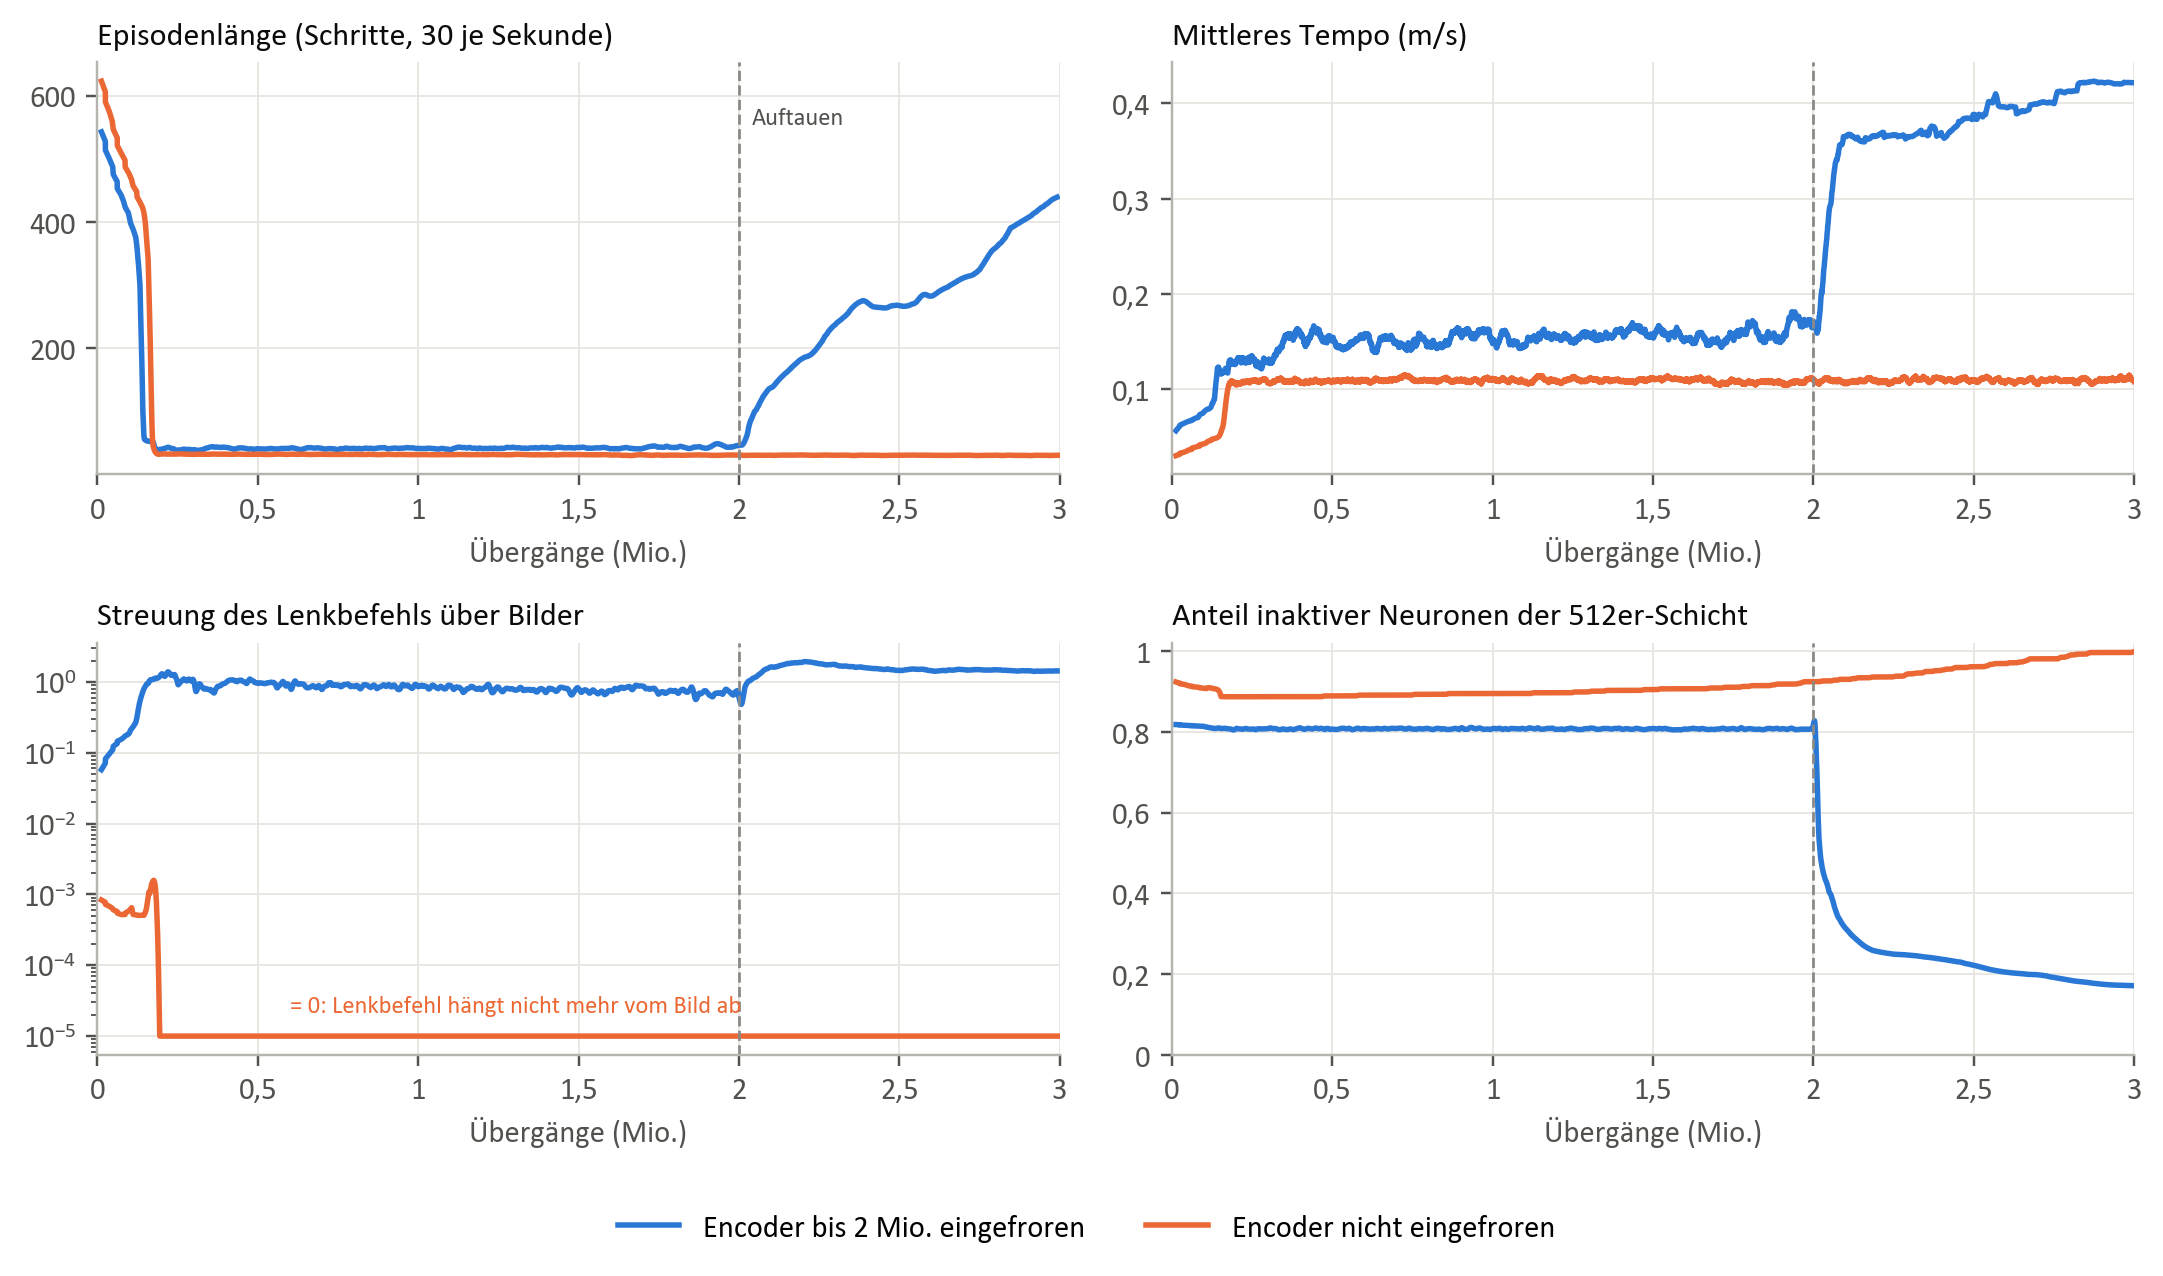
\includegraphics[width=\linewidth]{chapters/felix_teil/bilder/gegenversuch_einfrieren.png}
  \caption{Gegenversuch Einfrieren: identischer Aufbau mit eingefrorenem (blau) und nicht eingefrorenem Encoder (orange) auf \texttt{kurs\_A}.}
  \label{fig:gegenversuch_einfrieren}
\end{figure}

Ohne Einfrieren wird der Agent blind. Schon nach einer halben Million Übergängen hängt der Lenkbefehl nicht mehr vom Bild ab, und die 512er-Schicht stirbt bis zum Ende fast vollständig ab. Der Agent fährt keine Runde, die Episoden enden nach etwa einer Sekunde. Mit Einfrieren bleibt das Sehen erhalten; nach dem Auftauen steigen Episodenlänge und Tempo, und der Agent fährt nach \num{2.9}~Mio.\ Übergängen seine erste Runde.

Damit ist das Einfrieren als notwendig belegt. Ohne Schutz zerstört das \ac{RL} den vortrainierten Encoder in den ersten Hunderttausend Übergängen, bevor der Kopf gelernt hat, ihn zu nutzen.

\subsection{Der erste fahrende Kamera-Agent}
\label{sec:agent1}

Nach Behebung dieser Probleme gelingt mit Agent~1 das erste Training eines Kamera-Agenten, der zuverlässig Runden fährt.

\subsubsection{Genutzte Parameter}
\label{subsec:agent1_einstellungen}

Mit den Einstellungen aus Tabelle~\ref{tab:agent1_einstellungen} gelang das erste Training eines Kamera-Agenten, der zuverlässig Runden fährt.

Gegenüber den vorherigen Läufen wurden zwei Dinge geändert: Statt 64 laufen nur noch 4 parallele Umgebungen, wodurch der Erfahrungsspeicher je Umgebung 69 statt 4 Minuten Fahrt enthält, und die Faltungsschichten bleiben bis \num{0.3}~Mio.\ Übergänge eingefroren.

\begin{table}[htbp]
  \centering
  \caption{Einstellungen von Agent~1.}
  \label{tab:agent1_einstellungen}
  \small
  \begin{tabularx}{\linewidth}{@{}l X@{}}
    \toprule
    \textbf{Einstellung} & \textbf{Agent~1} \\
    \midrule
    Parallele Umgebungen                    & 4 \\
    Beobachtung                             & 3 Bilder à \num{250} $\times$ \num{150} Pixel, 256 Graustufen \\
    Darstellungen der Strecke               & 1 \\
    Vortraining                             & \ac{BC} auf \num{48000} Lehrerpaaren; übernommen: Faltungsschichten \\
    Eingefroren                             & Faltungsschichten bis \num{0.3}~Mio.\ Übergänge \\
    Batchgröße / Updates                    & 512 / 2 je Simulationsschritt (\num{0.5} je Übergang) \\
    Erfahrungsspeicher gesamt / je Umgebung & \num{500000} / \num{125000} Übergänge ($\approx$ \SI{69}{\minute} Fahrt) \\
    Lernrate / Diskontfaktor $\gamma$       & \num{5e-5} / \num{0.99} \\
    Episodenlänge                           & \SI{66.67}{\second}; in der Fortsetzung \SI{133.33}{\second} \\
    Übergänge im fertigen Modell            & \num{2.2}~Mio.\ (\num{1.2} + \num{1.0}) \\
    Durchsatz                               & $\approx$ 11 Übergänge/s (rund \SI{38}{\hour} je \num{1.5}~Mio.) \\
    \bottomrule
  \end{tabularx}
\end{table}

\subsubsection{Das Ergebnis}
\label{subsec:agent1_ergebnis}

Der erste erfolgreiche Agent fährt seine erste vollständige Runde nach rund \num{0.92}~Mio.\ Übergängen. Da das Training auf \num{1.5}~Mio.\ Übergänge ausgelegt ist und die Ergebnisse erstmals vielversprechend sind, wird es fortgesetzt: ausgehend vom Stand bei \num{1.2}~Mio.\ Übergängen um weitere \num{1.0}~Mio.\ Übergänge, mit doppelt so langen Episoden (\num{4000} statt \num{2000} Schritte). Längere Episoden setzen den Schwerpunkt auf stabiles Fahren, da der Agent mehr Runden am Stück fahren muss.

Dieser Agent lernt auf einer Strecke mit stets gleicher Darstellung. Abbildung~\ref{fig:agent1_verlauf} zeigt den Verlauf beider Trainingsabschnitte.

\begin{figure}[htbp]
  \centering
  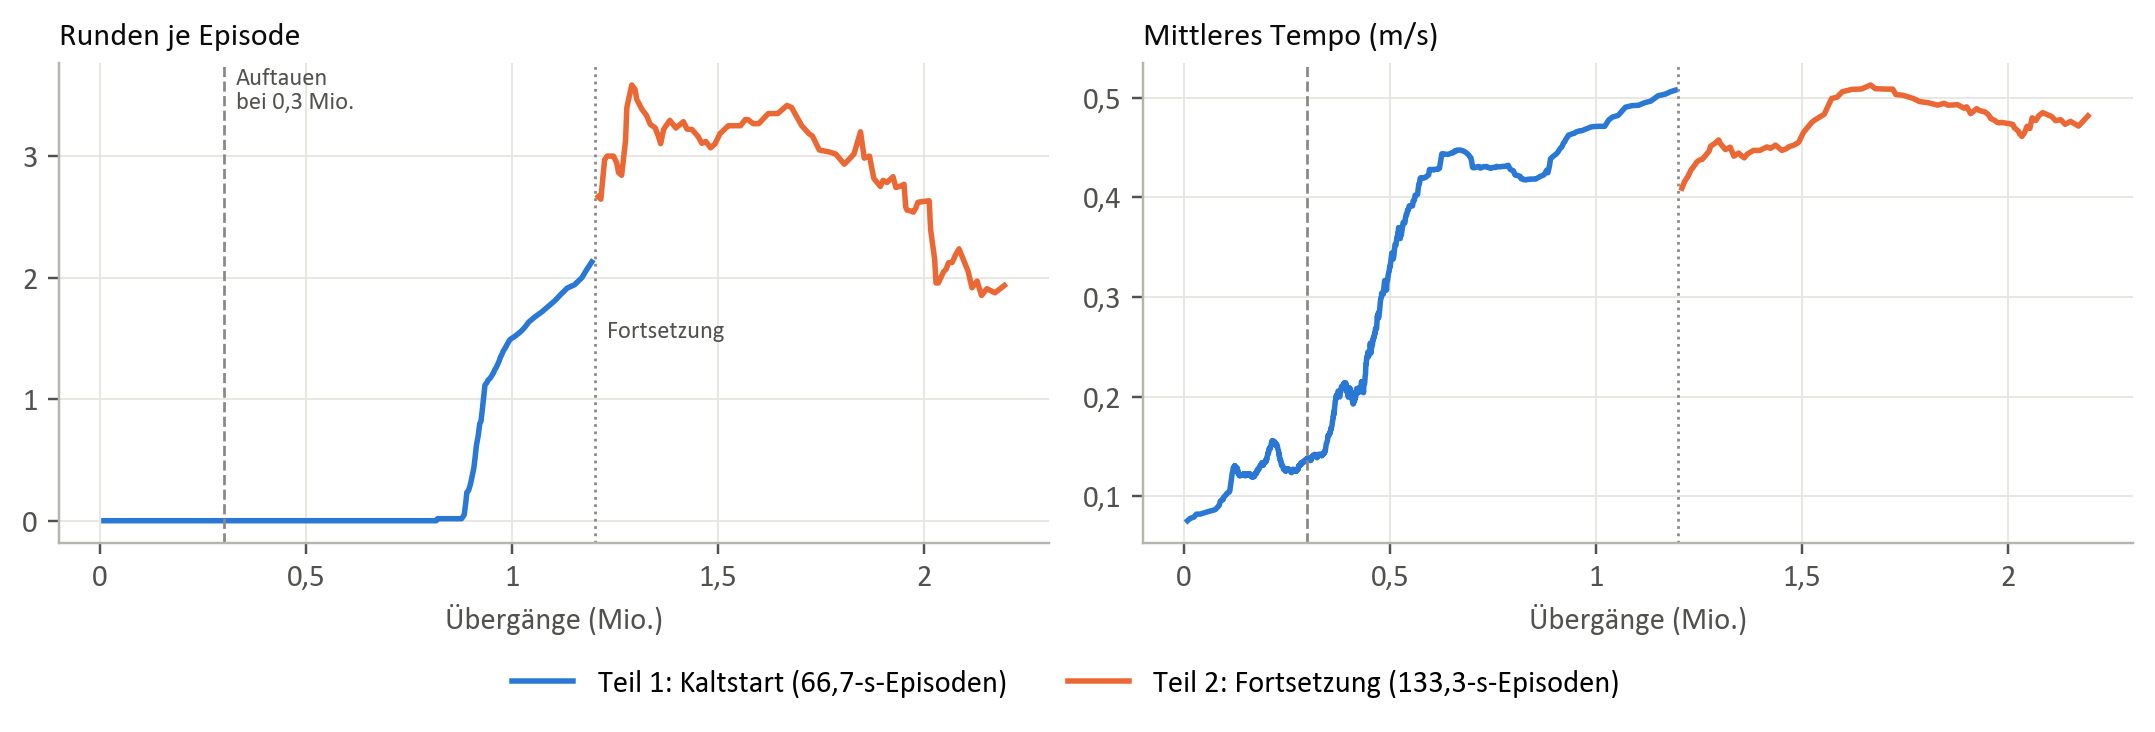
\includegraphics[width=\linewidth]{chapters/felix_teil/bilder/agent1_verlauf.png}
  \caption{Trainingsverlauf von Agent~1 (Werte mit Explorationsrauschen). Blau: erstes Training, orange: Fortsetzung mit doppelt so langen Episoden; gestrichelt: Auftauen der Faltungsschichten.}
  \label{fig:agent1_verlauf}
\end{figure}

Deterministisch gemessen, also ohne Explorationsrauschen und über zehn Episoden, fährt Agent~1 auf seiner Darstellung \num{6.4} Runden je Episode von \SI{66.67}{\second}, mit einer mittleren Geschwindigkeit von \SI{0.65}{\meter\per\second} und einer besten Runde von \SI{8.65}{\second}. Ca.\ \SI{10}{\percent} der Episoden enden mit einem Crash. Zum Vergleich fährt der zustandsbasierte Lehrer, der alle Größen exakt kennt, auf der gleichen Strecke etwa \SI{8.3}{\second} je Runde. Agent~1 ist also rund \SI{4}{\percent} langsamer, obwohl dieser die Lage und Bewegungen des Fahrzeugs aus \num{9} $\times$ \num{4} Pixeln ablesen muss. In Episoden von \SI{200}{\second} fährt er im Mittel \num{10.4} Runden mit einer besten Runde von \SI{8.59}{\second}. In 3 von 10 Episoden fährt er rund 20 Runden ohne Crash, \SI{70}{\percent} der langen Episoden enden jedoch vorzeitig. Der beste Bild-Agent der 2D-Umgebung schaffte unter vergleichbaren Bedingungen mit gestreuten Startpunkten \num{3.1} Runden.

Der kurze Einbruch zu Beginn der Fortsetzung in Abbildung~\ref{fig:agent1_verlauf} ist kein Verlernen. Stable-Baselines3 wählt in den ersten Schritten eines Laufs Zufallsaktionen, um den Speicher zu füllen; bei der Fortsetzung waren das \num{50000} Übergänge, in denen der Agent zufällig fuhr.

\paragraph{Ursache des Durchbruchs.}
Der Durchbruch dieses Agenten kann nicht eindeutig auf eine einzelne Änderung zurückgeführt werden. Gegenüber den vorherigen Läufen wird zum einen die Zahl der Umgebungen von 64 auf 4 reduziert, wodurch jede Umgebung einen größeren Anteil des Erfahrungsspeichers erhält, zum anderen werden erstmals die Faltungsschichten eingefroren. Damit wurde der Grundsatz verletzt, je Lauf nur eine Größe zu verändern.

Einen Hinweis liefert der vorherige Gegenversuch zum Einfrieren des Encoders (Abschnitt~\ref{sec:einfrieren}). Dort erblindet der Agent ohne Einfrieren, obwohl jede Umgebung mit \SI{104}{\minute} Fahrt über einen noch größeren Speicheranteil verfügt. Das spricht dafür, dass das Einfrieren den größeren Anteil am Durchbruch hatte. Für Agent~1 selbst ist es nicht belegt, da beide Änderungen nie getrennt untersucht wurden.

\subsubsection{Eine Einschränkung}
\label{subsec:agent1_einschraenkung}

Um zu prüfen, wie weit Agent~1 verallgemeinert, wurde er ohne weiteres Training auf derselben Streckenführung in anderen Darstellungen eingesetzt. Schon eine andere Darstellung genügt, damit er versagt. Auf jeder geprüften Darstellung fährt er null Runden, und jede Episode endet mit einem Crash, meist nach etwa einer Sekunde, ohne dass der Agent in Fahrt kommt. Das ist kein Fehler des Agenten, sondern eine Folge des Trainingsaufbaus. Über mehr als zwei Millionen Übergänge hinweg war das Kamerabild bis auf die Lage des Fahrzeugs identisch. Unter diesen Bedingungen ist Auswendiglernen die einfachste Lösung, und genau diese hat das Training gefunden.

Das deckt sich mit dem Befund aus Phase~1, dass bereits \SI{0.05}{\percent} abweichende Pixel eine Policy umwerfen können (Abschnitt~\ref{subsec:buffer}).

\subsection{Der zweite Agent}
\label{sec:agent2}

Dieser Abschnitt beschreibt den zweiten fahrenden Kamera-Agenten, im Folgenden Agent~2. Anders als Agent~1 soll er auch bei verändertem Aussehen der Strecke fahren. Dazu wechseln im Training die Darstellungen der Strecke, und der Encoder wird nicht auf die Aktionen eines Lehrers, sondern auf die Lage des Fahrzeugs vortrainiert.

\subsubsection{Verallgemeinern der Erscheinung}
\label{subsec:agent2_darstellung}

Das Problem von Agent~1 ist, dass er das Erscheinungsbild der Strecke und des Hintergrunds auswendig gelernt hat. Da der Agent auf einer realen Bahn fahren soll, muss dies behoben werden, da das reale Bild niemals exakt der Erscheinung der Simulation entsprechen wird. Untergrund, Licht, Unebenheiten und Farbunterschiede in der echten Strecke unterscheiden sich von der Simulation. Der Abstand zwischen der Darstellung im Training und der beim Einsatz heißt Domänenlücke (engl.\ \emph{domain gap}). Die übliche Abhilfe ist, im Training viele zufällig veränderte Darstellungen zu zeigen (\emph{Domain Randomization} \cite{tobin2017domain}).

Für die Randomisierung wurde ein Streckengenerator entwickelt, der Strecken aus Bildern der realen Carrera-Streckenteile zusammensetzt. Damit werden für dieselbe Streckenführung zwölf Darstellungen erzeugt, drei Untergründe kombiniert mit vier Helligkeitsstufen der Fahrbahn (Abbildung~\ref{fig:darstellungen}). Derselbe Generator erzeugt auch neue Streckenführungen, die in Abschnitt~\ref{sec:andere_strecken} verwendet werden.

\begin{figure}[htbp]
  \centering
  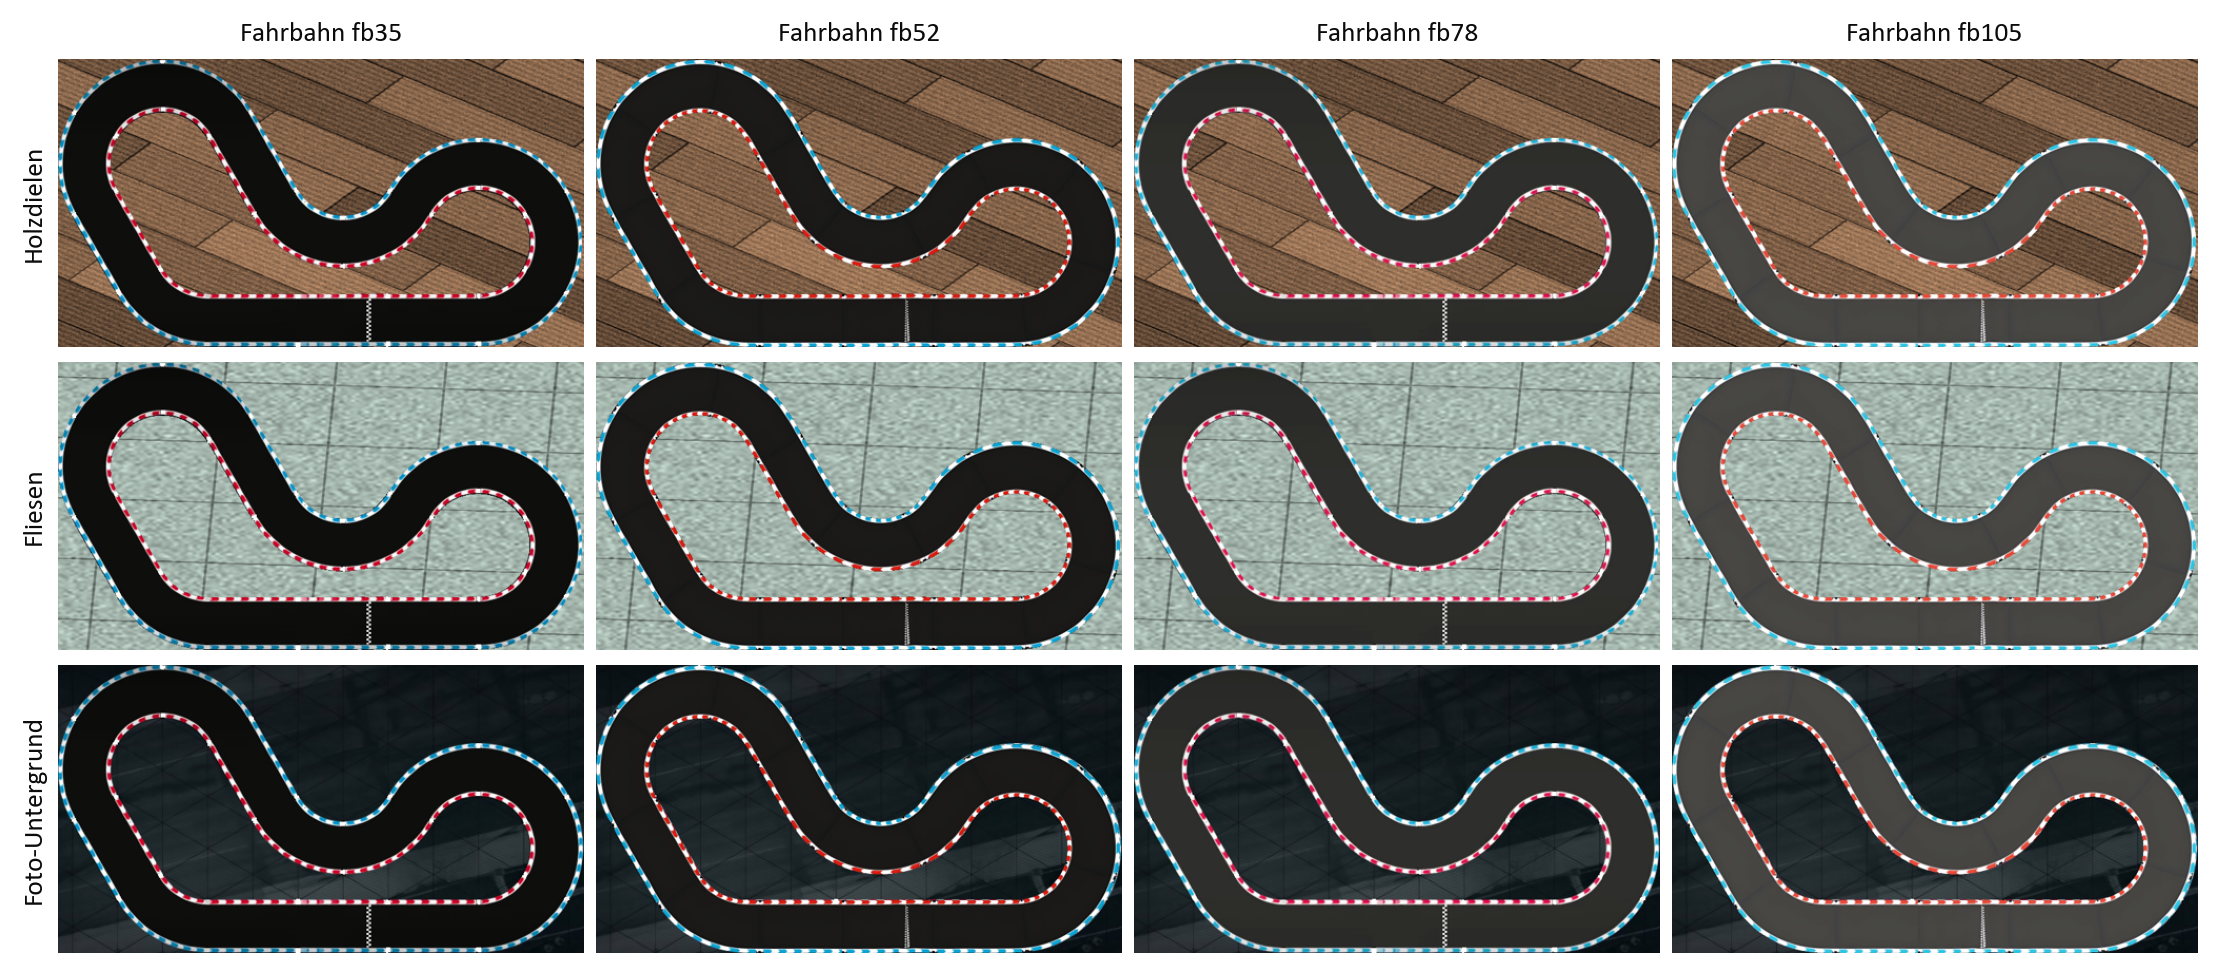
\includegraphics[width=\linewidth]{chapters/felix_teil/bilder/darstellungen.png}
  \caption{Die zwölf Darstellungen der Trainingsstrecke: drei Untergründe (Zeilen) und vier Helligkeiten der Fahrbahn (Spalten).}
  \label{fig:darstellungen}
\end{figure}

Weiterhin wird das Bild für Agent~2 auf vier Graustufen reduziert. Feine Unterschiede der Oberflächen verschwinden dadurch weitgehend, während Fahrbahn, Randsteine und Fahrzeug unterscheidbar bleiben. Zugleich lassen sich die Bilder mit \SI{2}{\bit} je Pixel im Erfahrungsspeicher ablegen.

\subsubsection{Das Training}
\label{subsec:agent2_training}

Agent~2 wird mit 16 parallelen Umgebungen trainiert. Der vortrainierte Encoder wird vollständig übernommen und bleibt bis 2~Mio.\ Übergänge eingefroren. Seine erste vollständige Runde fährt der Agent nach \num{3.9}~Mio.\ Übergängen. Das fertige Modell wurde über \num{14.5}~Mio.\ Übergänge in rund \SI{92}{\hour} trainiert.

Abbildung~\ref{fig:agent2_verlauf} zeigt den Trainingsverlauf. Die Kurven enthalten das Explorationsrauschen und sind über alle Darstellungen gemittelt. Sie liegen daher deutlich unter den deterministisch gemessenen Werten. Zwischen \num{4.4} und 5~Mio.\ Übergängen stieg der Verlust des Critics um das Hundertfache, und das Fahren brach vorübergehend ein. Zeitlich fällt das mit den ersten Runden zusammen, deren Bonus die Zielwerte des Critics sprunghaft erhöht. Der Encoder blieb dabei intakt, und der Agent erholte sich ohne Eingriff. Das ist ein Hinweis zu der in Phase~1 offenen Frage, warum \ac{SAC}-Läufe nach ihrem Höhepunkt einbrechen (Abschnitt~\ref{subsec:ppo_sac_vergleich}), aber keine Erklärung.

\begin{figure}[htbp]
  \centering
  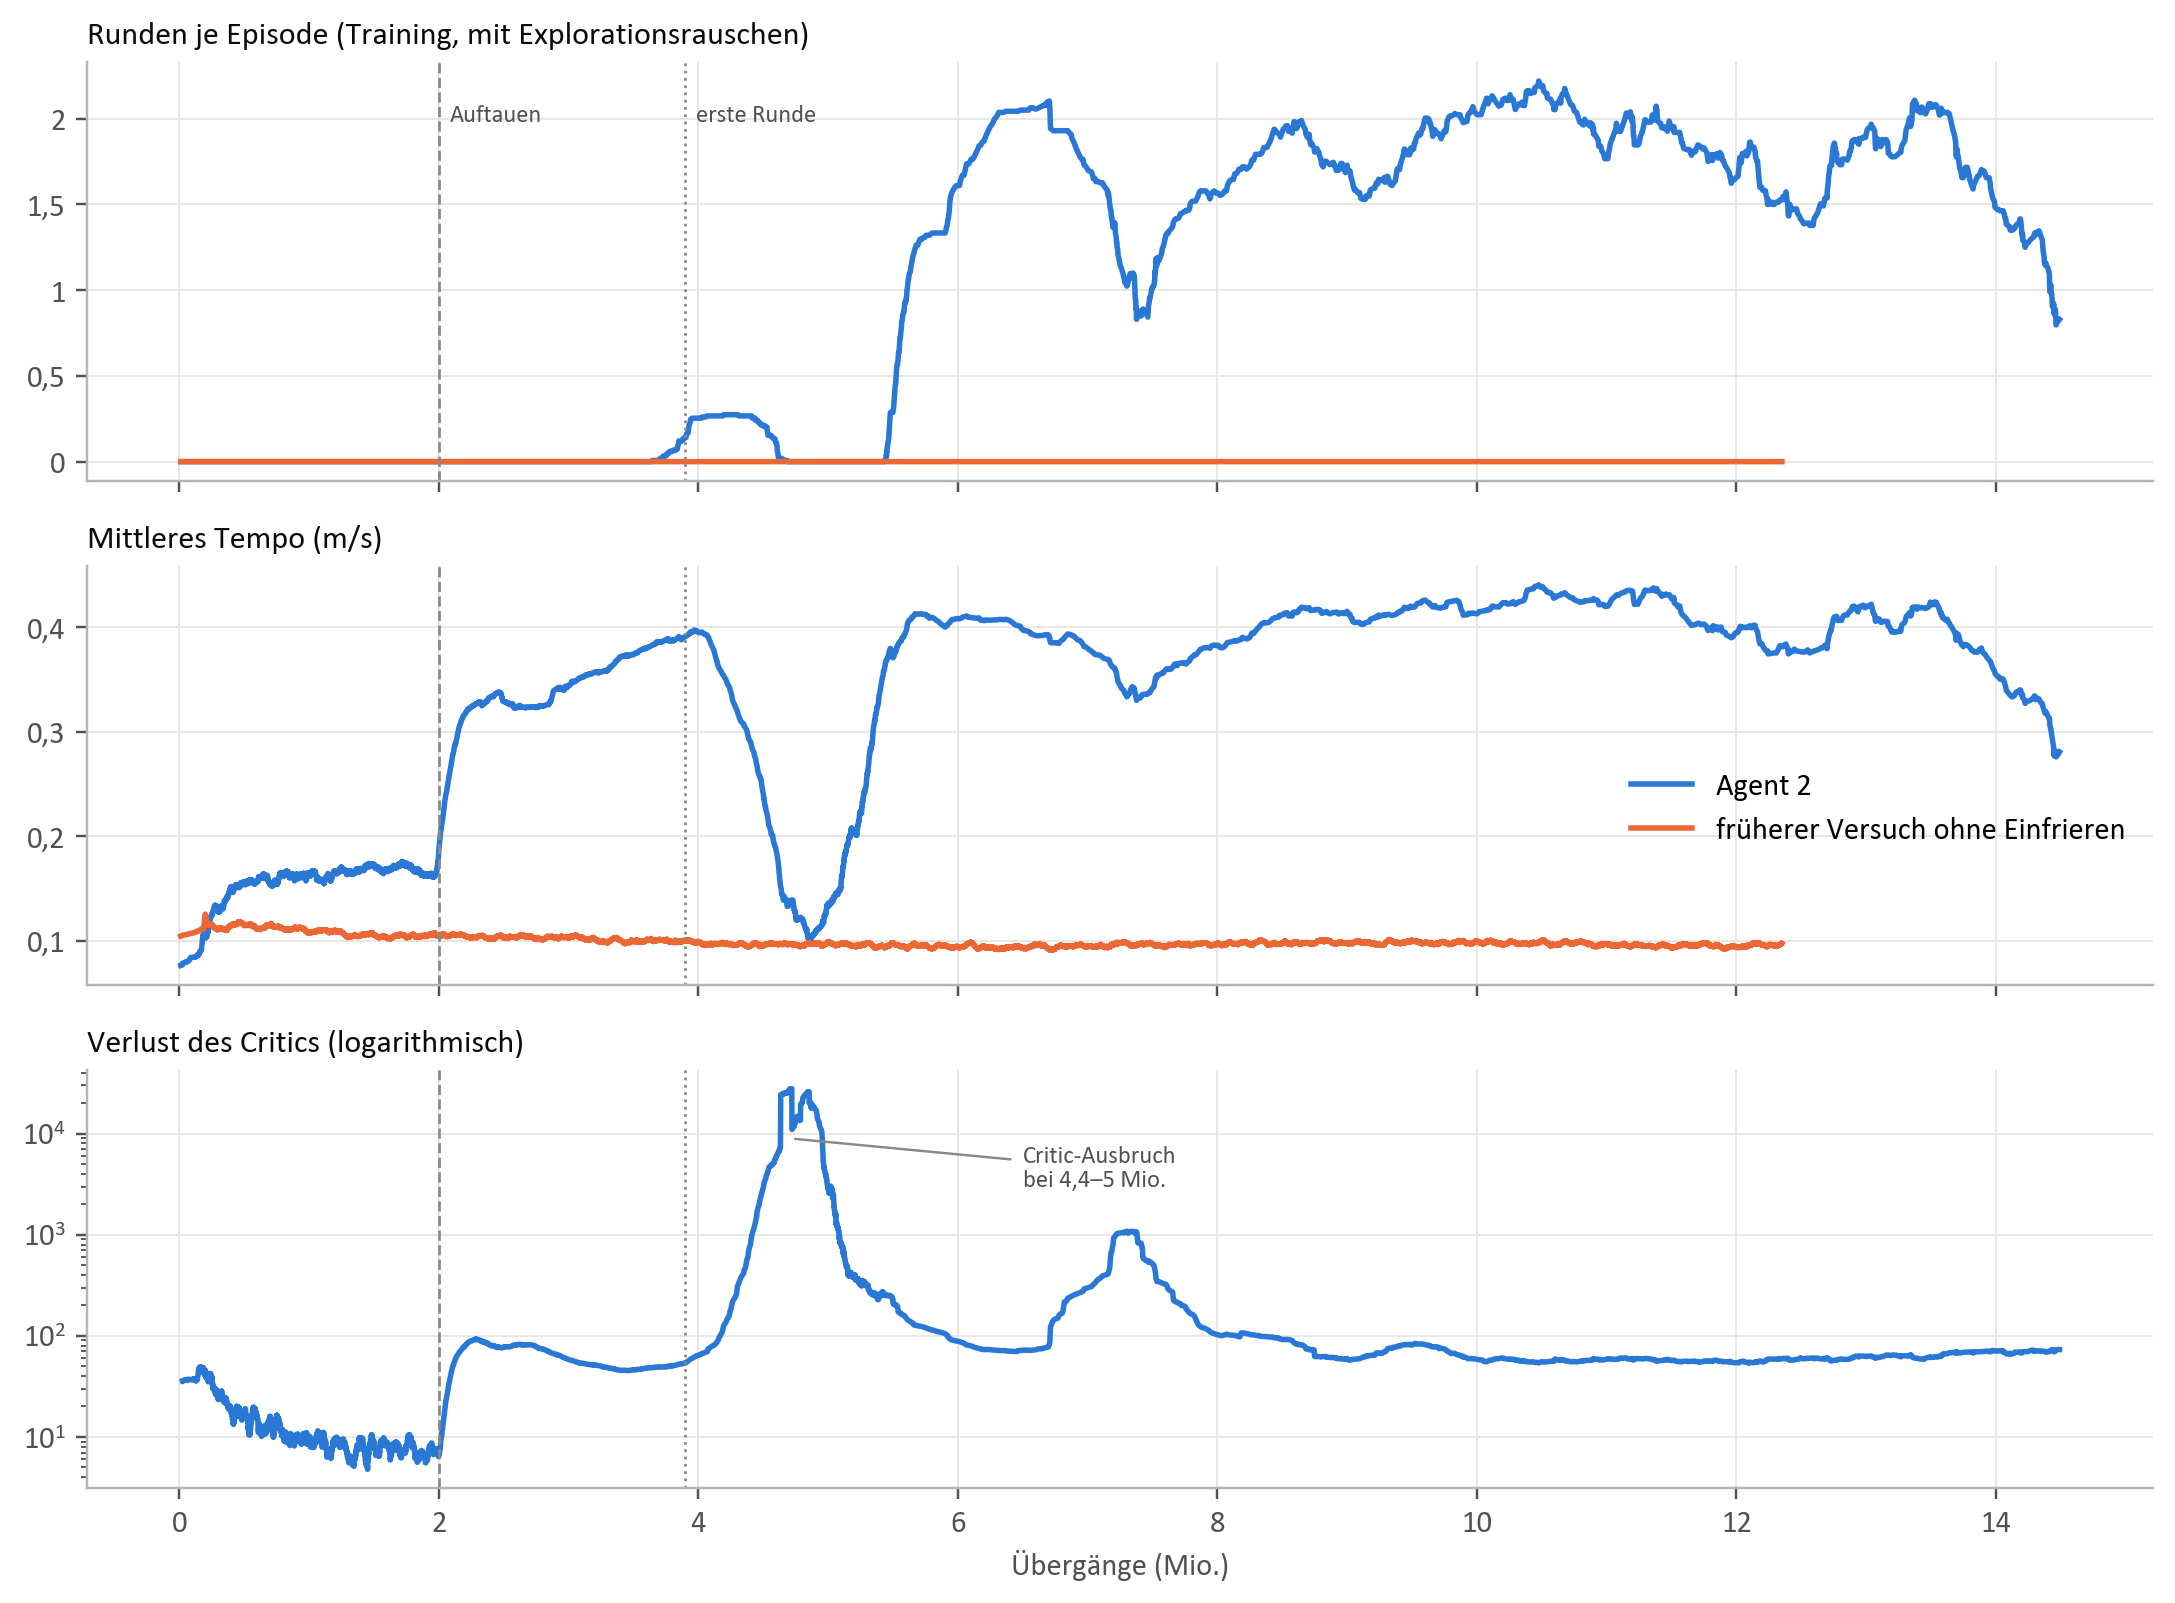
\includegraphics[width=\linewidth]{chapters/felix_teil/bilder/agent2_verlauf.png}
  \caption{Trainingsverlauf von Agent~2 im Vergleich zu einem früheren Versuch ohne Einfrieren (Werte mit Explorationsrauschen). Gestrichelt: Auftauen; gepunktet: erste vollständige Runde.}
  \label{fig:agent2_verlauf}
\end{figure}

\subsubsection{Das Ergebnis}
\label{subsec:agent2_ergebnis}

Abbildung~\ref{fig:agent2_darstellungen} zeigt das Ergebnis von Agent~2 nach \num{14.5}~Mio.\ Übergängen auf allen zwölf Darstellungen. Im Mittel fährt er \num{4.5} Runden je Episode bei einem Tempo von \SI{0.53}{\meter\per\second}. Die beste Runde dauert \SI{9.65}{\second}, und \SI{31}{\percent} der Episoden enden mit einem Crash. Auf allen zwölf Darstellungen fährt er Runden, auf sieben davon im Mittel mindestens fünf.

\begin{figure}[htbp]
  \centering
  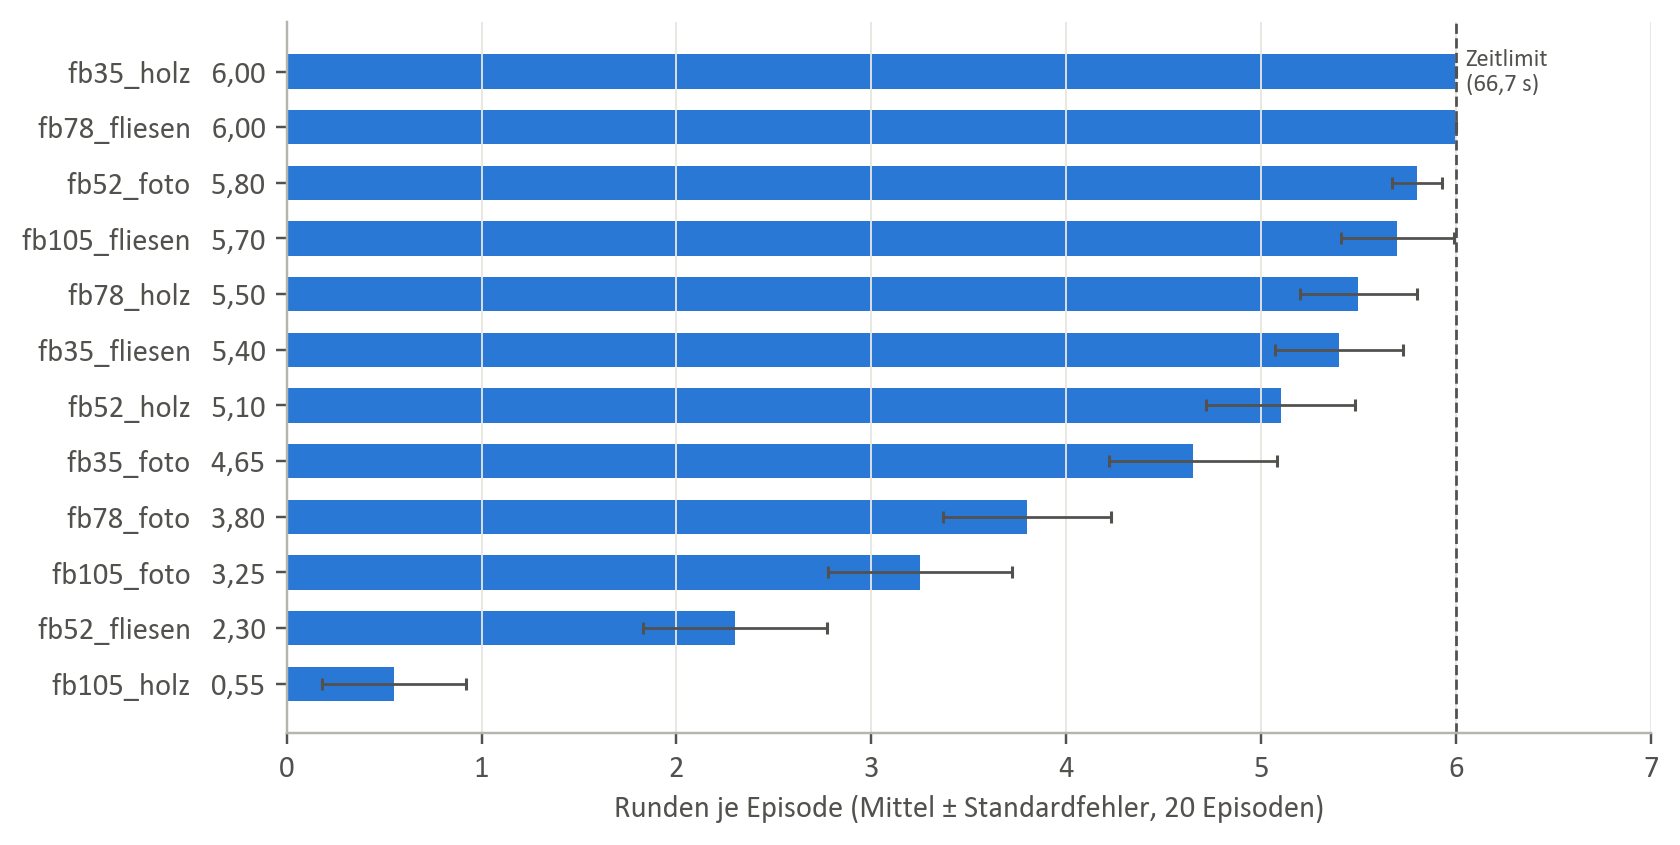
\includegraphics[width=0.9\linewidth]{chapters/felix_teil/bilder/agent2_darstellungen.png}
  \caption{Agent~2 auf den zwölf Darstellungen (je 20 Episoden à \SI{66.67}{\second}, deterministisch). Bei 6 Runden liegt das Zeitlimit. Die Werte der unteren Darstellungen sind Grenzfälle und schwanken zwischen Messungen; für \texttt{fb105\_holz} lagen sie in verschiedenen Messungen zwischen 0 und 4 Runden.}
  \label{fig:agent2_darstellungen}
\end{figure}

Drei Darstellungen erreichen bei \SI{66.67}{\second} das Zeitlimit von sechs Runden in jeder Episode, die Messung zeigt dort also nicht das Können, sondern die Episodenlänge. Mit \SI{200}{\second} langen Episoden fährt Agent~2 auf diesen drei Darstellungen \num{19} bis \num{19.7} Runden ohne einen einzigen Crash, im Mittel über alle zwölf \num{12.4} Runden.

\paragraph{Gegenprobe mit Agent~1.}
Als Gegenprobe wurde Agent~1 auf denselben zwölf Darstellungen gemessen: Er fährt auf keiner einzigen eine Runde und verlässt nach etwa einer Sekunde die Fahrbahn. Die Verallgemeinerung von Agent~2 ist damit nicht nur behauptet, sondern gegen ein Modell ohne Randomisierung geprüft.

\paragraph{Wo die schwachen Darstellungen scheitern.}
Auf den Darstellungen mit vielen Crashes verlässt der Agent fast immer in derselben Kurve die Fahrbahn. Der Hergang ist jedes Mal gleich: Innerhalb von \SI{0.3}{\second} wächst der Richtungsfehler von nahezu null auf über \SI{30}{\degree}, und der Gegenlenkbefehl kommt zu spät. Das Tempo ist dabei nicht die Ursache; auf einer sicher gefahrenen Darstellung durchfährt er dieselbe Kurve sogar schneller. Auch die Sichtbarkeit ist es nicht: Der Encoder liest die Lage auf der schwächsten Darstellung genauer ab als auf mancher sicher gefahrenen. Der Agent hat an dieser Stelle schlicht eine sehr kleine Reserve, sodass jede kleine Änderung der Eingabe das Ergebnis umkippen kann.

\paragraph{Feinere Graustufen.}
Dazu passt ein überraschender Befund. Wird das Kamerabild bei der Messung auf acht statt auf die trainierten vier Graustufen reduziert, sinkt die Crashrate auf der Darstellung \texttt{fb52\_fliesen} von \SI{80}{\percent} auf \SI{0}{\percent}, ohne jedes Nachtraining, auch mit 16 und 256 Stufen gab es keinen Crash. Der Agent verträgt also feinere Eingaben als die, auf denen er trainiert wurde. Für die Übertragung auf eine echte Kamera mit 256 Graustufen ist das die günstige Richtung.

\paragraph{Lohnt sich das lange Training?}
Agent~2 wurde nach \num{6.5} und nach \num{14.5}~Mio.\ Übergängen gemessen. Die Differenz von \num{0.54} Runden je Episode liegt innerhalb der Messunsicherheit (Standardfehler \num{0.61}), und die spätere Fassung ist nur auf sieben von zwölf Darstellungen besser. Sicher nachweisbar ist nur, dass sie schneller fährt, auf allen zwölf Darstellungen, mit kürzeren Rundenzeiten. Die zweite Hälfte des Trainings, rund \SI{50}{\hour}, hat also im Wesentlichen das Tempo verbessert, nicht die Zuverlässigkeit.

\subsection{Vergleich der beiden Modelle}
\label{sec:agentenvergleich}

Tabelle~\ref{tab:agentenvergleich} stellt Agent~1 und Agent~2 gegenüber. Die beiden Modelle lösen verschiedene Aufgaben und sind deshalb nicht direkt vergleichbar. Agent~1 fährt auf einer Darstellung und ist auf diese spezialisiert. Agent~2 dagegen fährt auf 12 unterschiedlichen Darstellungen.

\begin{table}[htbp]
  \centering
  \caption{Die beiden fahrenden Kamera-Agenten.}
  \label{tab:agentenvergleich}
  \small
  \begin{tabularx}{\linewidth}{@{}l X X@{}}
    \toprule
     & \textbf{Agent~1} & \textbf{Agent~2} \\
    \midrule
    Aufgabe                          & 1 Darstellung & 12 Darstellungen mit Bildstörungen \\
    Vortraining                      & \ac{BC} eines Lehrers (Fahrwissen) & Encoder für Versatz und Richtung (nur Sehwissen) \\
    Eingefroren                      & Faltungen bis \num{0.3}~Mio.\ Übergänge & gesamter Encoder bis 2~Mio.\ Übergänge \\
    Parallele Umgebungen             & 4 & 16 \\
    Graustufen                       & 256 & 4 \\
    Speicher je Umgebung             & \SI{69}{\minute} Fahrt & \SI{104}{\minute} Fahrt \\
    Übergänge bis zur ersten Runde   & \num{0.92}~Mio. & \num{3.9}~Mio. \\
    Übergänge im fertigen Modell     & \num{2.2}~Mio. & \num{14.5}~Mio. \\
    Runden je Episode (\SI{66.67}{\second}) & \num{6.4} auf seiner Darstellung, 0 auf den 12 anderen & \num{4.5} im Mittel über 12 \\
    Beste Runde                      & \SI{8.65}{\second} & \SI{9.65}{\second} \\
    Episoden mit Crash               & \SI{10}{\percent} & \SI{31}{\percent} \\
    \bottomrule
  \end{tabularx}
\end{table}

Neben der Aufgabe unterscheiden sich die beiden Agenten vor allem im Vortraining. Agent~1 hat Fahrwissen vom Lehrer geerbt, Agent~2 hat nur gelernt, wo das Auto auf der Bahn liegt, und das Fahren vollständig selbst gelernt. Dass Agent~2 viermal so viele Übergänge bis zur ersten Runde braucht, ist vor diesem Hintergrund und bei zwölffacher Aufgabe nicht überraschend.

\subsection{Test des zweiten Agenten auf anderen Streckenführungen}
\label{sec:andere_strecken}

Agent~2 fährt auf allen zwölf Darstellungen der Trainingsstrecke. Offen ist, ob er damit das Fahren an sich gelernt hat oder nur diese eine Streckenführung. Dazu wird er zunächst ohne weiteres Training auf neuen Streckenführungen getestet und anschließend auf zwei davon weitertrainiert.

\subsubsection{Test ohne Nachtraining}
\label{subsec:ohne_nachtraining}

Agent~2 wird ohne weiteres Training auf vier neuen Streckenführungen (\texttt{kurs\_A} bis \texttt{kurs\_D}) getestet, die mit dem Streckengenerator aus Abschnitt~\ref{subsec:agent2_darstellung} erzeugt wurden. Damit sich nur die Führung verändert und nicht gleichzeitig das Aussehen, wurden für \texttt{kurs\_A} dieselben zwölf Darstellungen erzeugt, auf denen Agent~2 trainiert wurde (Tabelle~\ref{tab:ohne_nachtraining}).

\begin{table}[htbp]
  \centering
  \caption{Agent~2 ohne Nachtraining (deterministisch).}
  \label{tab:ohne_nachtraining}
  \small
  \begin{tabular}{@{}l l l@{}}
    \toprule
    \textbf{Strecke} & \textbf{Darstellung} & \textbf{Runden je Episode} \\
    \midrule
    Original                              & trainiert (12) & \num{4.5} (\SI{66.67}{\second}) bzw.\ \num{12.4} (\SI{200}{\second}) \\
    Original                              & unbekannt      & \num{2.3} \\
    \texttt{kurs\_A}                      & trainiert (12) & \num{0.00} auf allen 12 \\
    \texttt{kurs\_A} bis \texttt{kurs\_D} & unbekannt      & \num{0.00} \\
    \bottomrule
  \end{tabular}
\end{table}

Eine unbekannte Darstellung der bekannten Strecke fährt der Agent noch mit \num{2.3} Runden. Eine unbekannte Streckenführung fährt er dagegen nicht, auch wenn sie in den bekannten Darstellungen gezeigt wird. Sein Verhalten auf \texttt{kurs\_A} ist dabei kein schlechteres Fahren, sondern eine Sättigung, voller Lenkeinschlag, Vollgas und Vollbremse gleichzeitig, ohne jede Korrektur. Es ist dasselbe Muster wie bei den blinden Agenten, obwohl der Encoder hier intakt ist.

Besonders aufschlussreich ist, dass \texttt{kurs\_A} die um \SI{180}{\degree} gedrehte Originalstrecke ist. Der Agent hat also nicht die Form der Strecke gelernt, sondern die Form in dieser Lage im Kamerabild. Für eine fest montierte Kamera über einer festen Strecke ist das kein Nachteil. Ein Agent, der jede beliebige Strecke fährt, entsteht so aber nicht.

\subsubsection{Weitertrainieren von Agent~2 gegen Neustart}
\label{subsec:weitertrainieren}

Da Agent~2 neue Streckenführungen ohne weiteres Training nicht fährt, wird untersucht, ob sein Vorwissen das Erlernen einer neuen Strecke zumindest beschleunigt. Dazu wird auf zwei Streckenführungen jeweils ein Weitertraining von Agent~2 mit einem Neustart verglichen:

\begin{description}
  \item[Weitertraining:] ausgehend vom fertigen Agent~2, also mit seinem Encoder und seiner Fahrweise;
  \item[Neustart:] ein neuer Agent mit demselben vortrainierten Encoder wie zu Beginn von Agent~2, eingefroren bis 2~Mio.\ Übergänge.
\end{description}

Als Strecken dienen \texttt{kurs\_A}, die gedrehte Originalstrecke, und \texttt{kurs\_D}, deren Fahrbahnfläche sich im Kamerabild nur zu \SI{21}{\percent} mit der Originalstrecke deckt. Gemessen wurde, nach wie vielen Übergängen die erste vollständige Runde fällt (Tabelle~\ref{tab:transfer}, Abbildung~\ref{fig:transfer}).

\begin{table}[htbp]
  \centering
  \caption{Übergänge bis zur ersten vollständigen Runde.}
  \label{tab:transfer}
  \small
  \begin{tabularx}{\linewidth}{@{}X l l l@{}}
    \toprule
    \textbf{Strecke} & \textbf{Weitertraining} & \textbf{Neustart} & \textbf{Ersparnis} \\
     & \textbf{(von Agent~2)} & \textbf{(nur Encoder)} & \\
    \midrule
    \texttt{kurs\_A} (Original, um \SI{180}{\degree} gedreht) & \num{2.81}~Mio. & \num{2.90}~Mio. & \SI{3}{\percent} \\
    \texttt{kurs\_D} (unähnlichste Führung)                   & \num{2.92}~Mio. & \num{3.29}~Mio. & \SI{11}{\percent} \\
    zum Vergleich: Agent~2 auf der Originalstrecke            & --              & \num{3.90}~Mio. & -- \\
    \bottomrule
  \end{tabularx}
\end{table}

\begin{figure}[htbp]
  \centering
  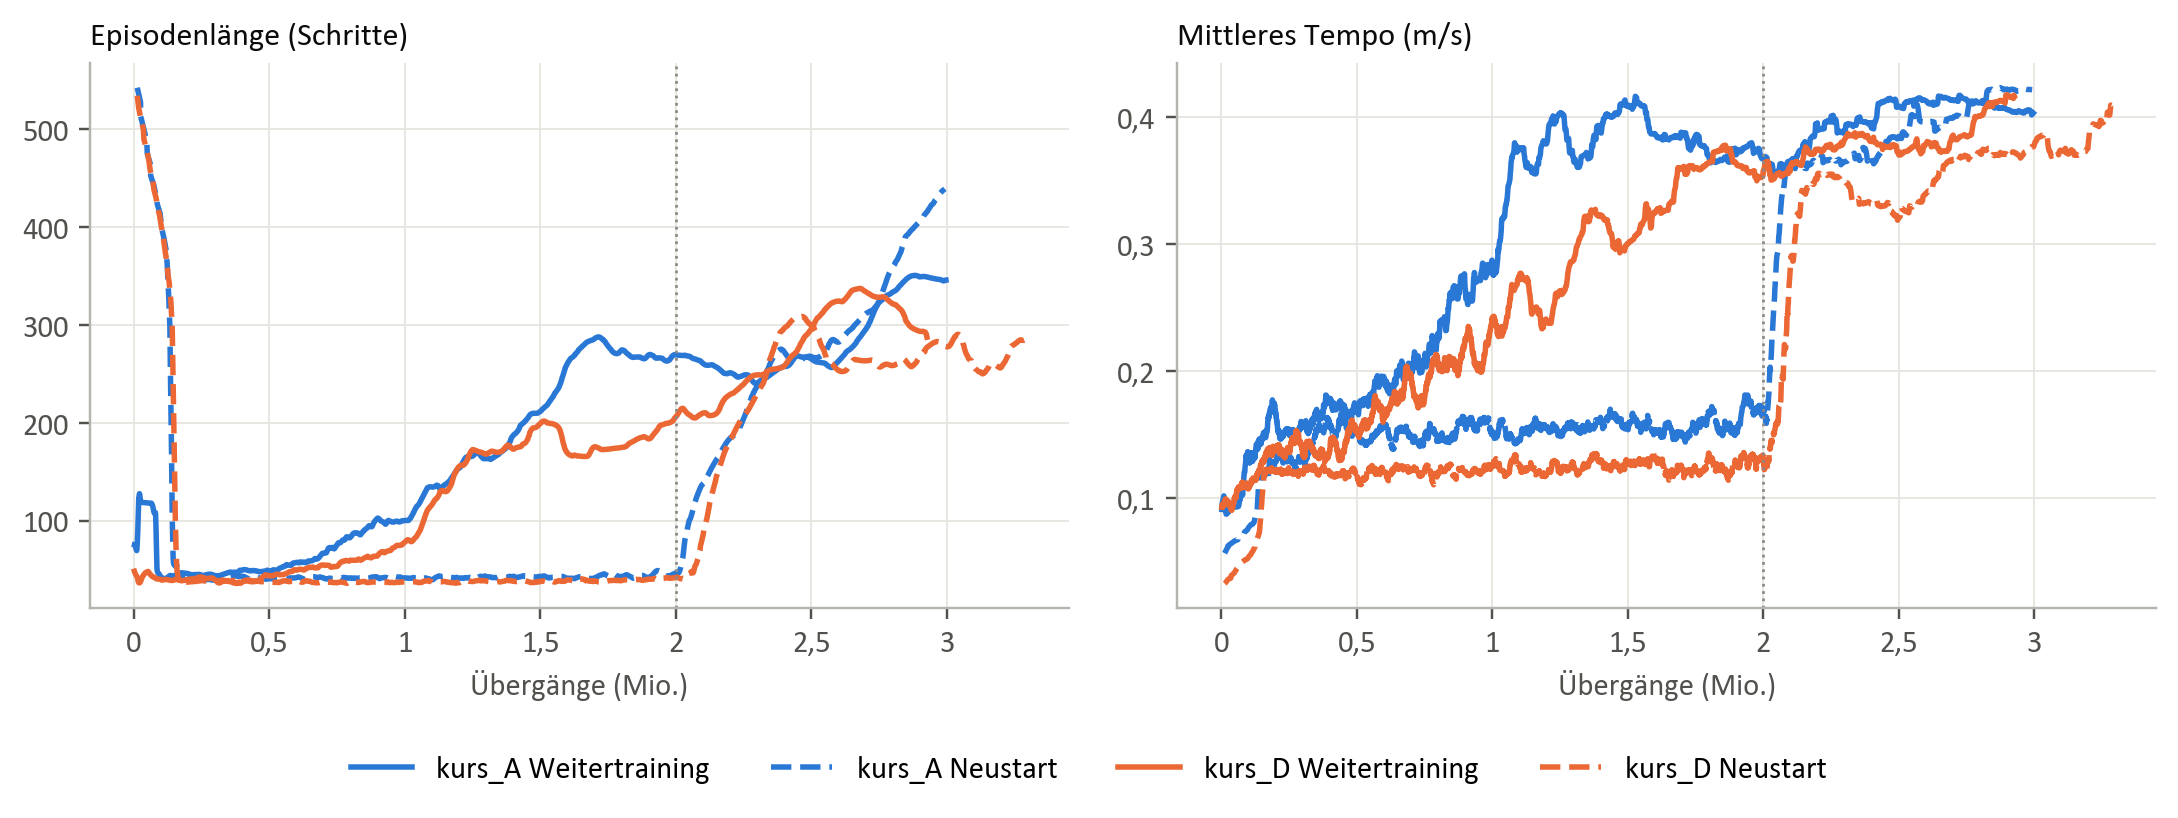
\includegraphics[width=\linewidth]{chapters/felix_teil/bilder/transfer.png}
  \caption{Weitertrainieren (durchgezogen) gegen Neustart (gestrichelt) auf \texttt{kurs\_A} (blau) und \texttt{kurs\_D} (orange). Bei 2~Mio.\ Übergängen wird der Encoder der Neustarts aufgetaut.}
  \label{fig:transfer}
\end{figure}

Das Vorwissen aus dem Training von Agent~2 bringt wenig: \SI{3}{\percent} auf \texttt{kurs\_A} und \SI{11}{\percent} auf \texttt{kurs\_D}. Da je Bedingung nur ein Lauf gefahren wird, kann ein Unterschied von \SI{3}{\percent} auch zufällig entstehen. Abbildung~\ref{fig:transfer} zeigt, woher der Unterschied kommt. Der weitertrainierte Agent lernt von Beginn an, weil sein Encoder nicht eingefroren werden muss, und ist nach \num{600000} bis \num{800000} Übergängen deutlich weiter. Sobald der Encoder des neu gestarteten Agenten bei 2~Mio.\ Übergängen aufgetaut wird, holt dieser den Rückstand innerhalb von etwa \num{600000} Übergängen auf.

Übertragbar ist damit das \emph{Sehen}, also die Fähigkeit, die Lage des Fahrzeugs im Bild abzulesen. Die \emph{Fahrweise} ist nicht übertragbar. Der Agent lernt nicht das allgemeine Fahren, sondern diese eine Strecke in dieser einen Kameraansicht.

Zwei Einschränkungen gelten für diesen Vergleich. Zum einen wird der Encoder des neu gestarteten Agenten auf Bildern der Originalstrecke trainiert. Beide Bedingungen bringen also Vorwissen von der Originalstrecke mit, und gemessen wurde genau der Beitrag der Fahrweise. Wie viel der Encoder auf einer fremden Strecke beiträgt, wurde nicht gemessen. Ein Neustart ganz ohne Encoder wurde dort nicht gefahren. Zum anderen musste der Neustart auf \texttt{kurs\_D} ab 3~Mio.\ Übergängen mit leerem Erfahrungsspeicher fortgesetzt werden, weil sich der gesicherte Speicher nicht laden ließ. Das hat ihn vermutlich gebremst; die \SI{11}{\percent} sind daher eher eine Obergrenze.
